\documentclass{article}
\usepackage[UTF8]{ctex}
\usepackage[T1]{fontenc}
\usepackage[utf8]{inputenc}
\usepackage{latexsym}
\usepackage{amsmath}
\usepackage{amssymb}
\usepackage[colorlinks, linkcolor = black]{hyperref}
\usepackage{float}
\usepackage[table, xcdraw]{xcolor}
\usepackage{listings}
\usepackage{graphicx}
\usepackage{booktabs}
\lstset{
    basicstyle = \ttfamily,
    keywordstyle = \bfseries,
    commentstyle = \textnormal,
    % linewidth = \linewidth,
    % xleftmargin = 0pt,
    % xrightmargin = 0pt,
    numbers = left,
    numberstyle = \textcircled,
    frame = none,
    escapeinside = ``,
    language = [x86masm]Assembler,
}
\usepackage{enumerate}
\usepackage{enumitem}
\setlist{
    leftmargin = .1\linewidth,
    % rightmargin = .1\linewidth,
    % label=\emph{\alph*}.
}

\title{Homework 4}
\author{PB17000297 罗晏宸}
\date{April 20 2020}

\begin{document}
\maketitle

\section{Exercise 3.15}
在这个练习中,我们将研究 Tomasulo 算法的各种变体在执行练习3.14中的循环\ref{3.14}时的表现。功能单元(FU)如下表所述。
\begin{table}[h]
    \centering
    \begin{tabular}{lccc}
        \toprule
        功能单元类型 & EX中的循环数 & 功能单元数 & 保留站数 \\
        \midrule
        整数         & 1            & 1          & 5        \\
        浮点加法器   & 10           & 1          & 3        \\
        浮点乘法器   & 15           & 1          & 2        \\
        \bottomrule
    \end{tabular}
\end{table}
\begin{figure}[h]
    \label{3.14}
    \centering
    \begin{lstlisting}[firstnumber = 0]
        DADDIU  R4, R1, #800 ; R4 = X 的上界
foo:    L.D     F2, 0(R1)    ; 载入 X(i)
        MUL.D   F4, F2, F0   ; 求乘积 a `$\times$` X(i)
        L.D     F6, 0($2)    ; 载入 Y(i)
        ADD.D   F6, F4, F6   ; 求和 a `$\times$` X(i) `$+$` Y(i)
        S.D     0(R2), F6    ; 存储 Y(i)
        DADDIU  R1, R1, #8   ; 递增 X 索引
        DADDIU  R2, R2, #8   ; 递增 Y 索引
        SGTIU   R3, R1, R4   ; 测试是否完成
        BEQZ    R3, foo      ; 如果没有完成则继续循环
    \end{lstlisting}
    \caption{练习3.14的循环}
\end{figure}
作出如下假设:
\begin{enumerate}[]
    \item[$\blacksquare$] 功能单元未实现流水化;
    \item[$\blacksquare$] 功能单元之间不存在转发,结果由公共数据总线(CDB)传送;
    \item[$\blacksquare$] 执行级(EX)既进行有效地址计算,又进行存储器访问,以完成载入和存储指令。因此,这个流水线为 IF/ID/IS/EX/WB;
    \item[$\blacksquare$] 载入指令需要一个时钟周期;
    \item[$\blacksquare$] 发射(IS)和写回(WB)结果级各需要一个时钟周期;
    \item[$\blacksquare$] 共有 5 个载入缓冲区槽和 5 个存储缓冲区槽;
    \item[$\blacksquare$] 假定“等于/不等于 0 时转移”(BNEZ)指令需要一个时钟周期。
\end{enumerate}
\begin{figure}[h]
    \centering
    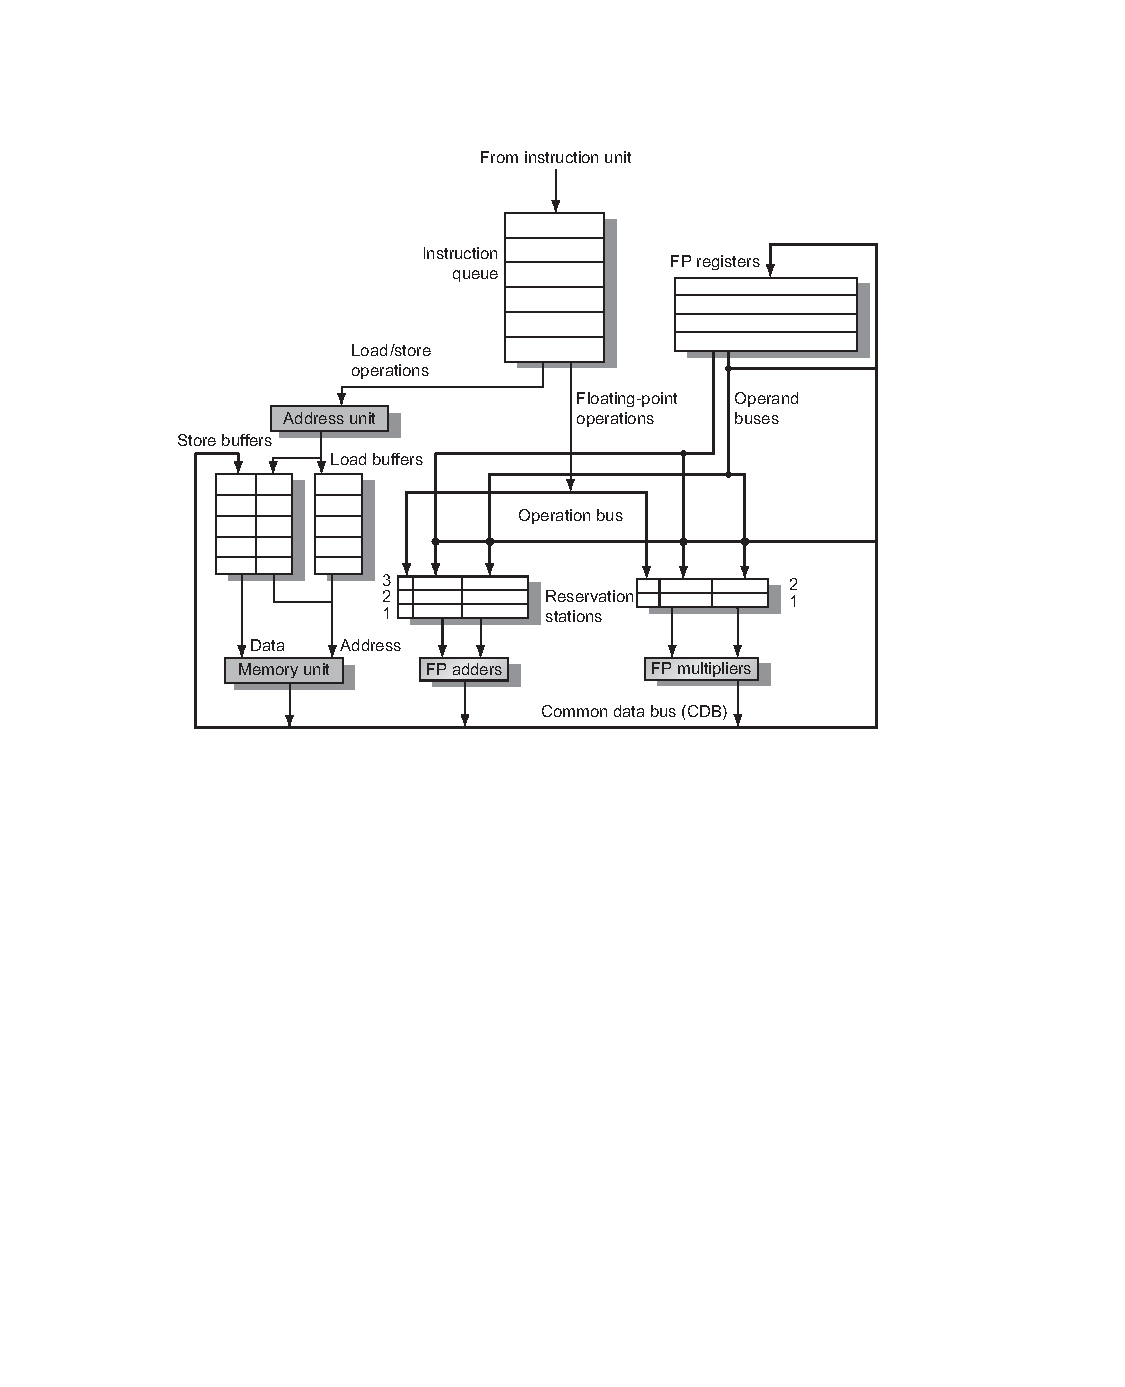
\includegraphics[scale = 1]{3-10.pdf}
    \caption{\textbf{使用 Tomasulo 算法的 MIPS 浮点单元的基本结构。指令由指令单元发送给指令队列,再按先入先出(FIFO)顺序从指令队列中发射出去。}保留站包括运算和实际操作数,还有用于检测和解决冒险的信息。载入缓冲区有 3 项功能:(1)保存有效地址的各个部分,直到计算完成;(2)跟踪正在等待存储器的未完成载入过程;(3)保存正在等待 CDB 的已完成载入过程的结果。与此类似,存储器缓冲区也有 3 项功能:(1)保存有效地址的各个部分,直到计算完成;(2)对于尚未完成、正在等待待存储数据值的存储过程,存储其目标存储器地址;(3)保存要存储的地址和数据值,直到存储器单元可用为止。来自 FP 单元或载入单元的所有结果都被放在 CDB 中,它会通向 FP 寄存器堆以及保留站和存储器缓冲区。 FP 加法器实现加法和减法, FP 乘法器完成乘法和除法}
    \label{3-4}
\end{figure}
\subparagraph{a} 对这个问题来说,使用图\ref{3-4}的单发射 Tomasulo MIPS 流水线,流水线延迟如上表所示。对于该循环的三个迭代,给出每个指令的停顿周期数以及每个指令在哪个时钟周期中开始执行(即,进入它的第一个 EX 周期)。每个循环迭代需要多少个时钟周期?以表格方式给出你的答案,表中应当具有以下列标头:
\begin{enumerate}[]
    \item[$\blacksquare$] 迭代(循环迭代数);
    \item[$\blacksquare$] 指令;
    \item[$\blacksquare$] 发射(发射指令的周期);
    \item[$\blacksquare$] 执行(执行指令的周期);
    \item[$\blacksquare$] 存储器访问(访问存储器的周期);
    \item[$\blacksquare$] 写 CDB(将结果写到 CDB 的周期);
    \item[$\blacksquare$] 注释(对指令正在等待的事件的说明)。
\end{enumerate}
在表中给出这个循环的三次迭代,可以忽略第一条指令。

\paragraph{解}
\subparagraph{a} 答案如表\ref{answer}所示。


第1次迭代的时钟周期数为 $31 - 1 + 1 = 31$,第2次迭代的时钟周期数为$46 – 10 + 1 = 37$,第3次迭代的时钟周期数为$61 – 19 + 1 = 43$。
\begin{table}[h]
    \label{answer}
    \centering
    \begin{tabular}{clcccc}
        \toprule
        迭代 & 指令                    & 发射 & 执行/存储器访问 & 写 CDB & 注释                \\
        \midrule
        1    & \lstinline[]!L.D     F2, 0(R1)!  & 1    & 2               & 3      &                     \\
        1    & \lstinline[]!MUL.D   F4, F2, F0!  & 2    & 4               & 19     & 等待\texttt{F2}写回 \\
        1    & \lstinline[]!L.D     F6, 0($2)!  & 3    & 4               & 5      &                     \\
        1    & \lstinline[]!ADD.D   F6, F4, F6!  & 4    & 20              & 30     & 等待\texttt{F4}     \\
        1    & \lstinline[]!S.D     0(R2), F6!  & 5    & 31              &        & 等待\texttt{F6}     \\
        1    & \lstinline[]!DADDIU  R1, R1, #8!  & 6    & 7               & 8      &                     \\
        1    & \lstinline[]!DADDIU  R2, R2, #8!  & 7    & 8               & 9      &                     \\
        1    & \lstinline[]!SGTIU   R3, R1, R4!  & 8    & 9               & 10     & 整型指令            \\
        1    & \lstinline[]!BEQZ    R3, foo!  & 9    & 11              &        & 等待\texttt{R3}     \\
        2    & \lstinline[]!L.D     F2, 0(R1)! & 10   & 12              & 13     & 等待跳转            \\
        2    & \lstinline[]!MUL.D   F4, F2, F0! & 11   & 19              & 34     & 乘法器忙            \\
        2    & \lstinline[]!L.D     F6, 0($2)! & 12   & 13              & 14     &                     \\
        2    & \lstinline[]!ADD.D   F6, F4, F6! & 13   & 35              & 45     & 等待\texttt{F4}     \\
        2    & \lstinline[]!S.D     0(R2), F6! & 14   & 46              &        &                     \\
        2    & \lstinline[]!DADDIU  R1, R1, #8! & 15   & 16              & 17     &                     \\
        2    & \lstinline[]!DADDIU  R2, R2, #8! & 16   & 17              & 18     &                     \\
        2    & \lstinline[]!SGTIU   R3, R1, R4! & 17   & 18              & 19     &                     \\
        2    & \lstinline[]!BEQZ    R3, foo! & 18   & 20              &        & 等待\texttt{R3}     \\
        3    & \lstinline[]!L.D     F2, 0(R1)! & 19   & 21              & 22     &                     \\
        3    & \lstinline[]!MUL.D   F4, F2, F0! & 20   & 34              & 49     & 乘法器忙            \\
        3    & \lstinline[]!L.D     F6, 0($2)! & 21   & 22              & 23     &                     \\
        3    & \lstinline[]!ADD.D   F6, F4, F6! & 22   & 50              & 60     & 等待\texttt{F4}     \\
        3    & \lstinline[]!S.D     0(R2), F6! & 23   & 61              &        & 等待\texttt{F6}     \\
        3    & \lstinline[]!DADDIU  R1, R1, #8! & 24   & 25              & 26     &                     \\
        3    & \lstinline[]!DADDIU  R2, R2, #8! & 25   & 26              & 27     &                     \\
        3    & \lstinline[]!SGTIU   R3, R1, R4! & 26   & 27              & 28     &                     \\
        3    & \lstinline[]!BEQZ    R3, foo! & 27   & 29              &        & 等待\texttt{R3}     \\
        \bottomrule
    \end{tabular}
    \caption{以表格形式呈现的答案,其中由于EX和MEM在同一个时钟周期内完成,所以合并了两个列标头}
\end{table}
\end{document}